

%%%%
%% Load the class. Put any options that you want here (see the documentation
%% for the list of options). The following are samples for each type of
%% thesis:
%%
%% Note: you can also specify any of the following options:
%%  logo: put a University of Edinburgh logo onto the title page
%%  frontabs: put the abstract onto the title page
%%  deptreport: produce a title page that fits into a Computer Science
%%      departmental cover [not sure if this actually works]
%%  singlespacing, fullspacing, doublespacing: choose line spacing
%%  oneside, twoside: specify a one-sided or two-sided thesis
%%  10pt, 11pt, 12pt: choose a font size
%%  centrechapter, leftchapter, rightchapter: alignment of chapter headings
%%  sansheadings, normalheadings: headings and captions in sans-serif
%%      (default) or in the same font as the rest of the thesis
%%  [no]listsintoc: put list of figures/tables in table of contents (default:
%%      not)
%%  romanprepages, plainprepages: number the preliminary pages with Roman
%%      numerals (default) or consecutively with the rest of the thesis
%%  parskip: don't indent paragraphs, put a blank line between instead
%%  abbrevs: define a list of useful abbreviations (see documentation)
%%  draft: produce a single-spaced, double-sided thesis with narrow margins
%%
%% For a PhD thesis -- you must also specify a research institute:
%\documentclass[phd,ilcc,twoside]{infthesis}

%% For an MPhil thesis -- also needs an institute
% \documentclass[mphil,ianc]{infthesis}

%% MSc by Research, which also needs an institute
% \documentclass[mscres,irr]{infthesis}

%% Taught MSc -- specify a particular degree instead. If none is specified,
%% "MSc in Informatics" is used.
% \documentclass[msc,cogsci]{infthesis}
 \documentclass[msc,ai,leftchapter,deptreport]{infthesis}  % for the MSc in Informatics

%% Master of Informatics (5 year degree)
% \documentclass[minf]{infthesis}

%% Undergraduate project -- specify the degree course and project type
%% separately
% \documentclass[bsc]{infthesis}
% \course{Artificial Intelligence and Psychology}
% \project{Fourth Year Project Report}

%% Put any \usepackage commands you want to use right here; the following is 
%% an example:
\usepackage{natbib}
\usepackage{braket}
\usepackage{amsmath}
\usepackage{caption}
\usepackage{mathtools}
\DeclarePairedDelimiter\floor{\lfloor}{\rfloor}


\usepackage{mathtools}
\newcommand\norm[1]{\left\lVert#1\right\rVert}

%% Information about the title, etc.
\title{Automatic Curriculum Learning for Deep Models Using Active Learning}
\author{Ian McWilliam}

%% If the year of submission is not the current year, uncomment this line and 
%% specify it here:
% \submityear{1785}

%% Optionally, specify the graduation month and year:
% \graduationdate{February 1786}

%% Specify the abstract here.
\abstract{%
    This 
}

%% Now we start with the actual document.
\begin{document}

%% First, the preliminary pages
\begin{preliminary}

%% This creates the title page
\maketitle

%% Acknowledgements
\begin{acknowledgements}
Many thanks
\end{acknowledgements}

%% Next we need to have the declaration.
\standarddeclaration

%% Finally, a dedication (this is optional -- uncomment the following line if
%% you want one).
% \dedication{To my mummy.}

%% Create the table of contents
\tableofcontents

%% If you want a list of figures or tables, uncomment the appropriate line(s)
% \listoffigures
% \listoftables

\end{preliminary}

%%%%%%%%
%% Include your chapter files here. See the sample chapter file for the basic
%% format.


\chapter{Introduction}

\textit{Supervised learning} is the area of machine learning in which algorithms learns the relationship between a set of input features and corresponding `ground truth' labels, the ultimate goal being to construct a predctive model of the relationships between the inputs and the labels in order to predict the labels of future, unseen input samples. Deep learning models perform this task by building hierarchical representations of the input features throughout a multitude of layers, often using feature maps such as convolutions or recurrent layers to construct complex representations of the inputs. When training a deep model a standard methodology is \textit{gradient descent}, which calculates the gradient of a chosen error function with respect to the free parameters of the model so as to tune the parameters in a way that will minise this error function on the training set of input-label pairs. A popular variant of the gradient descent algorithm is \textit{mini-batch stochastic gradient descent}, which uniformly samples mini-batches of a preset size from the available training data, performing a gradient descent update on each batch until the all training samples have been selected, then repeating until the network converges to a solution. Sampling uniformly from the training data ensures that the mini-batch gradient is an unbiased estimation of the gradient over the whole training set, however the estimation can exhibit high variance. In this paper we analyse approaches for augmenting mini-batch stochastic gradient descent (SGD), using methods inspired by two areas of study; \textit{active learning} and \textit{curriculum learning}. 

Active learning is generally used when there is a prohibitive cost to obtaining labels for supervised learning; in such cases it is desirable to know which samples will lead to the greatest best improvement in algorithm performance, selected from a set of unlabeled candidate samples. As such, there is a rich literature in active learning detailing how to choose the most informative samples, in particular using \textit{acquisition functions} to select which sample(s) to label and use for training. While active learning is usually employed to reduce labeling costs and speed up learning, curriculum learning explores the hypothesis that the overall accuracy of the network can be improved by presenting the training data to the algorithm in a meaningful order. Inspired by the way in which humans and animals learn, REF BENGIO suggest learning can be improved by emphasising easier concepts earlier on in training before introducing difficult samples, or by emphasising more difficult training samples later in training. In their paper REF BENGIO for example, the authors use a the `Geometric Shapes' dataset, consisting of images of geometric shapes of different complexities, to show that by initially training on `easy', regular shapes, test classification accuracy is improved. 

The substantial challenge with curriculum learning however is that in many domains however it is challenging to identify a clear delineation between `easy' and `hard' samples through which to implement curriculum learning; in this paper we propose that the methodologies developed for the active learning approach are well suited to estimating the difficulty of training samples, allowing the automatic construction of learning curricula that will improve the training of deep networks on a wide range of tasks. Specifically, the approach set out in this paper modifies the SGD algorithm by, instead of sampling with uniform probability, sampling training examples proportionally to some measure of `difficulty', as derived from an active learning style acquisition function metric. We test our methods on three image classification datasets; MNIST, CIFAR 10 and the GeoShapes dataset (a geometric shapes classification dataset with an established curriculum baseline), exploring a range of active learning metrics as well as several curriculum construction methods. Our results show consistent performance against a uniform sampling baseline, with significant reductions in test set error, robust to different network architectures, datasets and curriculum methodologies. The output of this work is a set of flexible methods for improving deep models in a wide range of tasks, as well as an investigation of how using the difficulty and uncertainty of training samples affect learning performance. 

In the next section we will introduce in more detail active and curriculum learning, exploring the link between the two approaches and the sometimes contradictory hypotheses they pose. We will then discuss related work where the authors implement similar methods for improving algorithm performance through biasing learning towards certain training samples throughout training. We will then lay out the experimental methodologies and datasets used in the paper before presenting and analysing the results of the tests and concluding with a discussion and suggestions for further work.

\chapter{Background}\label{ch:background}

\section{Supervised Learning}
Machine learning is the field of study concerned with building algorithmic systems that can automatically infer patterns and relationships in data. While machine learning has several main subfields, for example reinforcement \cite{sutton1998introduction} and unsupervised learning \cite{hastie2009unsupervised}, the most commonly studied area of the field is arguably \textit{supervised} learning. Supervised learning is characterised by learning a function that maps inputs to outputs (or `labels'), using a \textit{training set} of example input-output pairs \cite{Witten2011}, (supervised learning has previously been referred to as ``learning from examples'' \cite{cohn1994improving}). The training set, which we will denote by $\mathcal{T}$, consists of a number of inputs-output pairs: $\mathcal{T} = \{(x_1,y_1),(x_2,y_2),...(x_N,y_N)\}$, where $N$ is the number of examples in the training set. We will refer to an input-output pair from the training set as a `sample' or an `example' interchangeably. Concretely, the goal of supervised learning is to find a function $f : X \rightarrow Y$, where $X$ denotes the input space and $Y$ the output space, so as to minimize the \textit{generalization error} of the function \cite{murphy2012machine}. The generalization error is defined as the expected error of the function averaged over future input-output samples \cite{murphy2012machine}, where the error is defined using a loss function $L:Y \times Y \rightarrow \mathbb{R}$, such that $L(f(x_i),y_i)$ gives the error of the function on the input-output pair $\{x_i,y_y\}$. Generalization error can therefore be defined as $\mathbb{E}_{X\times Y}(L(f(x),y))$; as finding a closed form solution for the generalization error is generally intractable, it is usually approximated using the empirical error on a held out \textit{test set} of samples that were not used when fitting the function \cite{murphy2012machine}. Using a test set of $M$ input-output examples, we therefore approximate the generalization error as $\frac{1}{M}\sum_{i=1}^{M} L(f(x_i),y_i)$. A supervised learning algorithm is a method for fitting the function $f$ using the training set $\mathcal{T}$, usually by minimizing the loss of the function over the input-output samples in the training set \cite{murphy2012machine}, the process of fitting the function to the training data is referred to as \textit{training}. In order to avoid \textit{overfitting}, where the function has a low error on the training set but a high generalization error\footnote{More specifically, overfitting refers to the situation where the function has a low error on the training set and a higher generalization error than a similar function with a higher error on the training set.}, the loss function often includes regularization terms that penalize function complexity, or the range of functions that can be fitted by the algorithm is constrained \cite{Theodoridis2009}. Furthermore, in addition to a training set and test set, a \textit{validation set} of samples is often used to monitor the function error on samples outwith the training set during training, in order to measure whether or not the function is overfitting \cite{Witten2011}. 

\section{Deep Learning}
\textit{Deep learning}, as applied in the supervised learning setting, refers to algorithms which model the relationships in the training set using complex, hierarchical representations of the data, usually doing so using multiple `deep' layers, as well as feature maps such as convolutions or recurrent layers \cite{lecun2015deep}. Deep learning models fit functions by passing the input signals through several layers of transformations, multiplying the signal by parameterised weights and then passing the weighted signal through non-linear \textit{activation functions} \cite{Witten2011}. The combined model of weights and transformations is referred to as a `deep network', or `deep neural network', as a result of similarities to the functionalities of neurons in brain \cite{hinton2005kind}. This approach allows the algorithm to transform the input space in order to make the network outputs closely match the output, with the weight parameters being tuned throughout training in order minimise the network loss on the training set. Deep learning has been the subject of much research in recent years, showing state of the art performance in a range of domains including image recognition and natural language processing \cite{lecun2015deep} \cite{bengio2012practical}.

\subsection{Feedforward Networks}
Arguably the simplest example of a deep network is a \textit{feedforward network}, usually consisting of an input layer, an output layer and several intermediate `hidden' layers \cite{Witten2011}. There are a variety of `hyper-parameters' that must be set when implementing a feedforward network, or any deep model, for example the architecture (i.e. number of hidden layers and the number of nodes each layer contains), learning rate and chosen activation functions \cite{Witten2011}.

In classification problems, where the aim is to classify an input $x$ into one of several possible classes, the output activation function used is the softmax function \cite{Theodoridis2009}, which maps the output vector to a vector of probabilities, summing to one. Denoting by $\mathbf{h}$ the signal forward propagated through the network to the output layer, the final output vector of the network is then given by $softmax(\mathbf{h})$, where:
\begin{equation}
softmax(\mathbf{h})_i = \frac{e^{h_i}}{\sum_{c=1}^Ce^{h_c}},
\end{equation}
where $C$ is the number of possible class labels. The loss function typically used to train such networks is the \textit{cross-entropy} loss function, defining the output vector of the network for input sample $x$ by $f(x) = \tilde{\mathbf{y}}$, cross-entropy error is defined as follows:
\begin{equation}
cross entropy(\tilde{\mathbf{y}},\mathbf{y}) = - \sum_{c=1}^{C} y_{c} log(\tilde{y}_{c}).
\end{equation}
In several of the experiments in this report we will use feedforward networks for image classification, using a softmax output layer and cross-entropy error as the chosen loss function. 

\subsection{Convolutional Networks}\label{sec:convnets}
The state of the art deep models for image recognition are \textit{convolutional networks} \cite{lecun2015deep} \cite{bengio2012practical}. Convolutional layers pass filters of a predetermined size over an image, allowing for weight sharing between nearby pixels and the subsequent extraction of visual features \cite{lecun2015deep}. Usually, multiple convolutional layers are used in order to extract a hierarchical representation of different features, before the signal is flattened to a vector output and passed through the softmax function for classification. Convolutional layers are often followed by \textit{max pooling} layers \cite{nagi2011max}, which downsample the the signal into a lower dimension, and also \textit{batch normalisation} layers \cite{ioffe2015batch}, which normalises the signal as it propagates through the network. 

\section{Stochastic Gradient Descent}
The standard method for training deep models is \textit{gradient descent (GD)} \cite{Witten2011} \cite{Theodoridis2009}, an optimization algorithm which varies the parameters in the model depending on the gradient of the chosen error function with respect to the model parameters. Defining the current weight parameters of the network by $\theta_{old}$, the updated weight after gradient descent as $\theta_{new}$ and the loss function of the model on the training set $\mathcal{T}$ by $L(\theta)$, we update the weight parameters by performing a gradient descent update as follows:
\begin{equation}
\theta_{new} = \theta_{old} + \Delta \theta,
\end{equation}
where
\begin{equation}
\Delta \theta = -\alpha \frac{\partial L(\theta)}{\partial\theta} |_{\theta_{old}}.
\end{equation}
$\alpha$ in this case is the pre-set \textit{learning rate} \cite{Witten2011}, controlling the step-size of the gradient descent update. To implement GD it is necessary to calculate the gradient of the error function with respect to the parameters of the model, usually this is done layer by layer, starting with the output layer, in a method referred to as \textit{backpropogation} \cite{lecun1988theoretical}. 

One of the drawbacks of gradient descent is that calculating this gradient over the entire training set can be very computationally expensive, particularly when dealing with large training sets; to address this issue a variant of GD, \textit{stochastic gradient descent (SGD)}, is often used \cite{shamir2013stochastic}. With SGD, instead of calculating the error gradient over the entire training set, only one sample is used to calculate the gradient and update the model parameters. Alternatively a selection or `mini-batch' of training samples may be used to calculate the gradient, in which case the optimization algorithm is referred to as \textit{mini-batch stochastic gradient descent} \cite{ruder2016overview}. To implement mini-batch SGD, batches of samples are selected uniformly from the training data, usually without replacement, and gradient descent updates are performed using the sample in the batch. This is then repeated until all of the training samples have been used in a batch; a complete pass through the training data is referred to as an \textit{epoch}, and the number of training epochs is set as a parameter of the experiment \cite{ruder2016overview}. 

It can be shown that that SGD and mini-batch SGD produce an unbiased estimate of the error gradient \cite{shamir2013stochastic}, with various convergence proofs showing that SGD will eventually converge to an optimal solution under certain conditions \cite{shamir2013stochastic}. There are many adaptations to `vanilla' SGD, for example momentum based methods \cite{sutskever2013importance} and other more sophisticated optimization algortihms which build on SGD to result in better and quicker fitting of the model parameters. In this paper we will employ the ADAM optimiser \cite{kingma2014adam}, the details of which are laid out in Algorithm 1 of \cite{kingma2014adam}. 




\section{Curriculum Learning}
When training a deep model, or indeed any supervised learning algorithm, one usually trains the model over the entire training set throughout the entirety of training. When using stochastic gradient descent for example, all epochs would typically consist of a full pass through all available training samples. \textit{Curriculum learning}, as introduced in \cite{Bengio2009}, hypothesises that model performance can be improved by instead training on samples in a meaningful order, with the order defining a `curriculum'. The motivation stems from the way in which humans and other animals  learn, usually beginning with easy concepts before moving onto more complex facets of the area of study. The same principle can be applied to training deep models, and the authors of \cite{Bengio2009} suggest that, by initially training only on `easy' samples, one can reduce overall generalization error. 

While the term curriculum learning in the machine learning setting may be a relatively new one, the concept was arguably introduced with Elman's 1993 paper ``Learning and development in neural networks: the importance of starting small'' \cite{ELMAN199371}. In this paper the author demonstrates in a language modeling task that inhibiting the memory of the network in the early stages of learning, so that it can only analyse a small subset of the training set, ultimately improves performance. The author motivates the method by analysing the learning dynamics of connectionist networks, specifically the sensitivity of the overall model to the early stages of training and the subsequent implications for what data should be used in these early epochs. Interestingly, the author suggests motivations for beginning training with either `easy' or `hard'/'noisy' samples. In the case of using easy samples, he argues that this will prevent the network from falling into ``early commitment to erroneous hypotheses'', instead enabling it to learn broader concepts at the key early stage of training that will act as ``scaffolding'' for more complex concepts.  Conversely, he also suggests that using harder/noisier samples may also prevent the network from reaching such erroneous hypotheses, as the high variance in noisier samples will lead to less consistent gradient descent updates and prevent the networks weights from converging to an area of parameter space from which it will be difficult to exit in the later stages of training. This dynamic, wherein initialising learning with either easy and hard samples somewhat paradoxically seems to improve learning in both cases, is something which will be revisited throughout this report.

The authors of \cite{Bengio2009} also offer several theoretical justifications for curriculum learning, for example comparing the technique to \textit{continuation methods} \cite{Allgoer1980}. It is proposed that the easier samples represent a smoother, more convex version of the error space of the overall problem, and that, by training on easier samples, the parameters of the model are effectively initialized into an area of parameter space closer to the global optimum. This argument is similar to that of unsupervised pre-training \cite{erhan2009difficulty} which again has been shown to lead to better generalized models by initializing the parameters into parts of the error space closer to the global optimum \cite{bengio2012practical}. Comparisons have also been drawn between curriculum learning and \textit{transfer learning} \cite{pan2010survey}, with the easier samples being seen as a separate task that the model is trained on, before using the weights for a different task (i.e. the harder samples) as in transfer learning \cite{weinshall2018curriculum}.  

The example given in \cite{Bengio2009}  for curriculum learning is the `Geometric Shapes' dataset \cite{GeoShapes}, an image classification task where a network attempts to classify whether or a not an image shows a rectangle, ellipse or triangle. In this case there is a natural subset of `easy' samples; specifically squares (i.e. regular rectangle), circles (regular ellipses) and equilateral triangles. The authors show that, by training initially on only the regular shapes, then transitioning to training on harder shapes, the test set performance is significantly improved compared to training only on the hard shapes for the entirety of training. One issue with this study is that it can be argued that the curriculum trained model has seen more samples overall than the baseline, as the curriculum model is trained on both an `easy' training set and a `hard' training set, whereas the baseline is trained only on the hard training set. A better baseline therefore is a model trained uniformly on the union of the easy and hard training sets. While the authors do comment on this issue, and claim that the curriculum method still outperforms uniform sampling from the combined training set, some of the results we will set out in this paper did not reach the same conclusions. 

Curriculum learning is similar in concept to \textit{self-paced learning} \cite{kumar2010self}. In a paper of the same title \cite{kumar2010self}, the authors train a latent SSVM model \cite{felzenszwalb2008discriminatively} by adding a regularization term to the objective function that indicates whether or not a sample is `easy' or note, depending on how well the current model parameters correctly classify the sample. Using this approach they limit the number of training samples used for parameter updates, as governed by a weight parameter that is annealed throughout training until all training samples are considered. They test their method on a variety of tasks including natural language processing and image classification. While the self-paced learning (SPL) method is tested for the SSVM model in \cite{kumar2010self}, an exploration of SPL as applied to convolution networks is laid in \cite{avramova2015curriculum}. The author applies SPL and a variant defined as `Self-Paced Learning with Diversity (SPLD)' \cite{jiang2014self} which expands the SPL method to emphasise a diverse representation of samples. 

The author of \cite{avramova2015curriculum} tests various curriculum methods on the CIFAR 10 image classification dataset, interestingly, similar to the remarks mentioned above in \cite{ELMAN199371}, the author found that training on samples with \textit{decreasing} difficulty outperformed the standard curriculum of training on samples with increasing difficulty. However, the author reports that little overall improvements were seen in any of the curriculum methods compared to standard training procedure using the entire training set. There are various examples of curriculum learning being applied in areas where the learning problem can be split into discrete `tasks'. For example in \cite{pentina2015curriculum}, the authors use an animal image classification dataset that has been manually annotated with a perceived `easiness' score. The authors divide the dataset into five equal tasks depending on difficulty score, demonstrating that their curriculum method outperforms a standard multi-task learning algorithm. The authors of \cite{louradour2014curriculum} also find a natural curriculum in a handwritten text line recognition task, finding that by first training on short sequences of text, before progressing to to the longer sequences significantly accelerates the training time of of a recurrent neural network \cite{mikolov2010recurrent} model for text recognition. More recent applications of curriculum learning include \cite{weinshall2018curriculum}, where the authors provide a theoretical study of how curriculum learning affects the convergence of stochastic gradient descent, as well as implementing a curriculum using transfer learning by using a model trained on a separate task to construct a curriculum for an image classification task, finding that the curriculum improves performance. The authors also test the effect of using an ``anti-curriculum'', where training progress from difficult to easy samples, as in \cite{avramova2015curriculum}, however they find this significantly underperformance the baseline, as illustrated in Figure \ref{TransferExample}, taken from Figure 3b of \cite{weinshall2018curriculum}. 

\begin{figure}[h!]
\centering
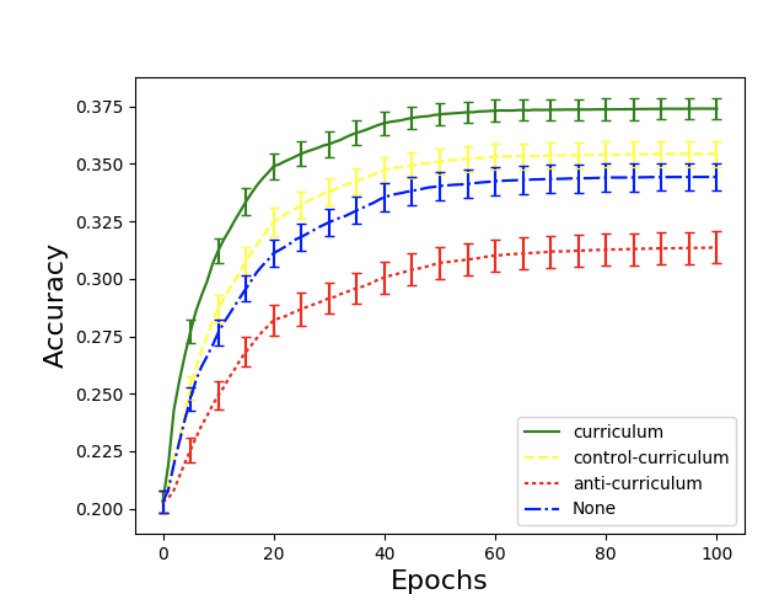
\includegraphics{TransferLearningCurricExample.png}
\caption{Figure 3b from  \cite{weinshall2018curriculum}, test classification accuracy of a convolutional network trained using various curriculum methods on the CIFAR 100 dataset \cite{krizhevsky2009learning}. The curriculum method trains on progressively more difficult samples, while the anti-curriculum method trains on progressively easier samples. The control-curriculum is trained using a random curriculum to control for differences in training between the curriculum methods and the baseline.}
\label{TransferExample}
\end{figure}

While the number of studies implementing curriculum learning methods is increasing, a key difficulty in constructing a curriculum is that it is often very difficult to delineate between `easy' and `difficult' samples \cite{Bengio2009}, particularly for large datasets where manually annotating the difficulty of the each sample is infeasible. It is also an open question as to how best to construct a learning curriculum, given a measure of sample difficulty, in particular given the aforementioned questions around whether or not training should progress through increasingly difficult or easy samples. A key issue therefore is that of exploring methods for automating the construction of learning curricula, and it is towards this goal that this paper contributes; specifically investigating how active learning methods (introduced in the next section) can aid such curriculum construction. In Chapter \ref{Related Work}, we will discuss a variety of other studies that have implemented methods for automated curriculum construction. We first however introduce \textit{active learning}, including some of the methods we will use to estimate sample difficulty and construct learning curricula in Chapters \ref{ch:BootstrappedActiveCurricula} and \ref{ch:DAC}.


\section{Active Learning}\label{Background_ActiveLearning}
A key component in any supervised learning effort is labeled data; in many domains it is relatively easy and cheap to obtain a large number of training samples, however in others it can be far more costly, particularly acquiring accurate labels. In medical image analysis for example one may require a domain expert to spend significant time analysing each image before assigning label, or in document tagging it can take time to read a document and assign a topic label. It can therefore be very useful for a designer to understand which samples they should go to the effort of acquiring, labeling and feeding into their chosen learning algorithm. A field of study that attempts to address this is \textit{active learning} \cite{settles2012active} \cite{cohn1994improving} \cite{cohn1996active}, which studies methods for choosing, often from a pool of unlabeled candidate samples, which sample should be labeled and used to train the model. Generally the efficacy of an active learning method is measured by how much the chosen samples improve the model performance, compared to if samples were instead selected randomly \cite{settles2012active}.

Figure \ref{ActiveLearningExample}, taken from Figure 1 of \cite{settles2012active} shows a typical active learning cycle; a machine learning model is trained on the current set of labeled training data, $\mathcal{L}$, the model then ``queries'' an ``oracle'', in this case a human annotator, for the labels of one or more samples from a pool of unlabeled  samples, denoted $\mathcal{U}$. The queried samples are then labeled and added to $\mathcal{L}$, at which point the model is retrained using the expanded training set and the cycle reiterates until training is stopped. Note that, as well as pool based query strategies, some active learning methods may enable the model to query samples from the entire input space, as opposed to being limited to a pool of unlabeled samples \cite{settles2012active}.

\begin{figure}[h!]
\centering
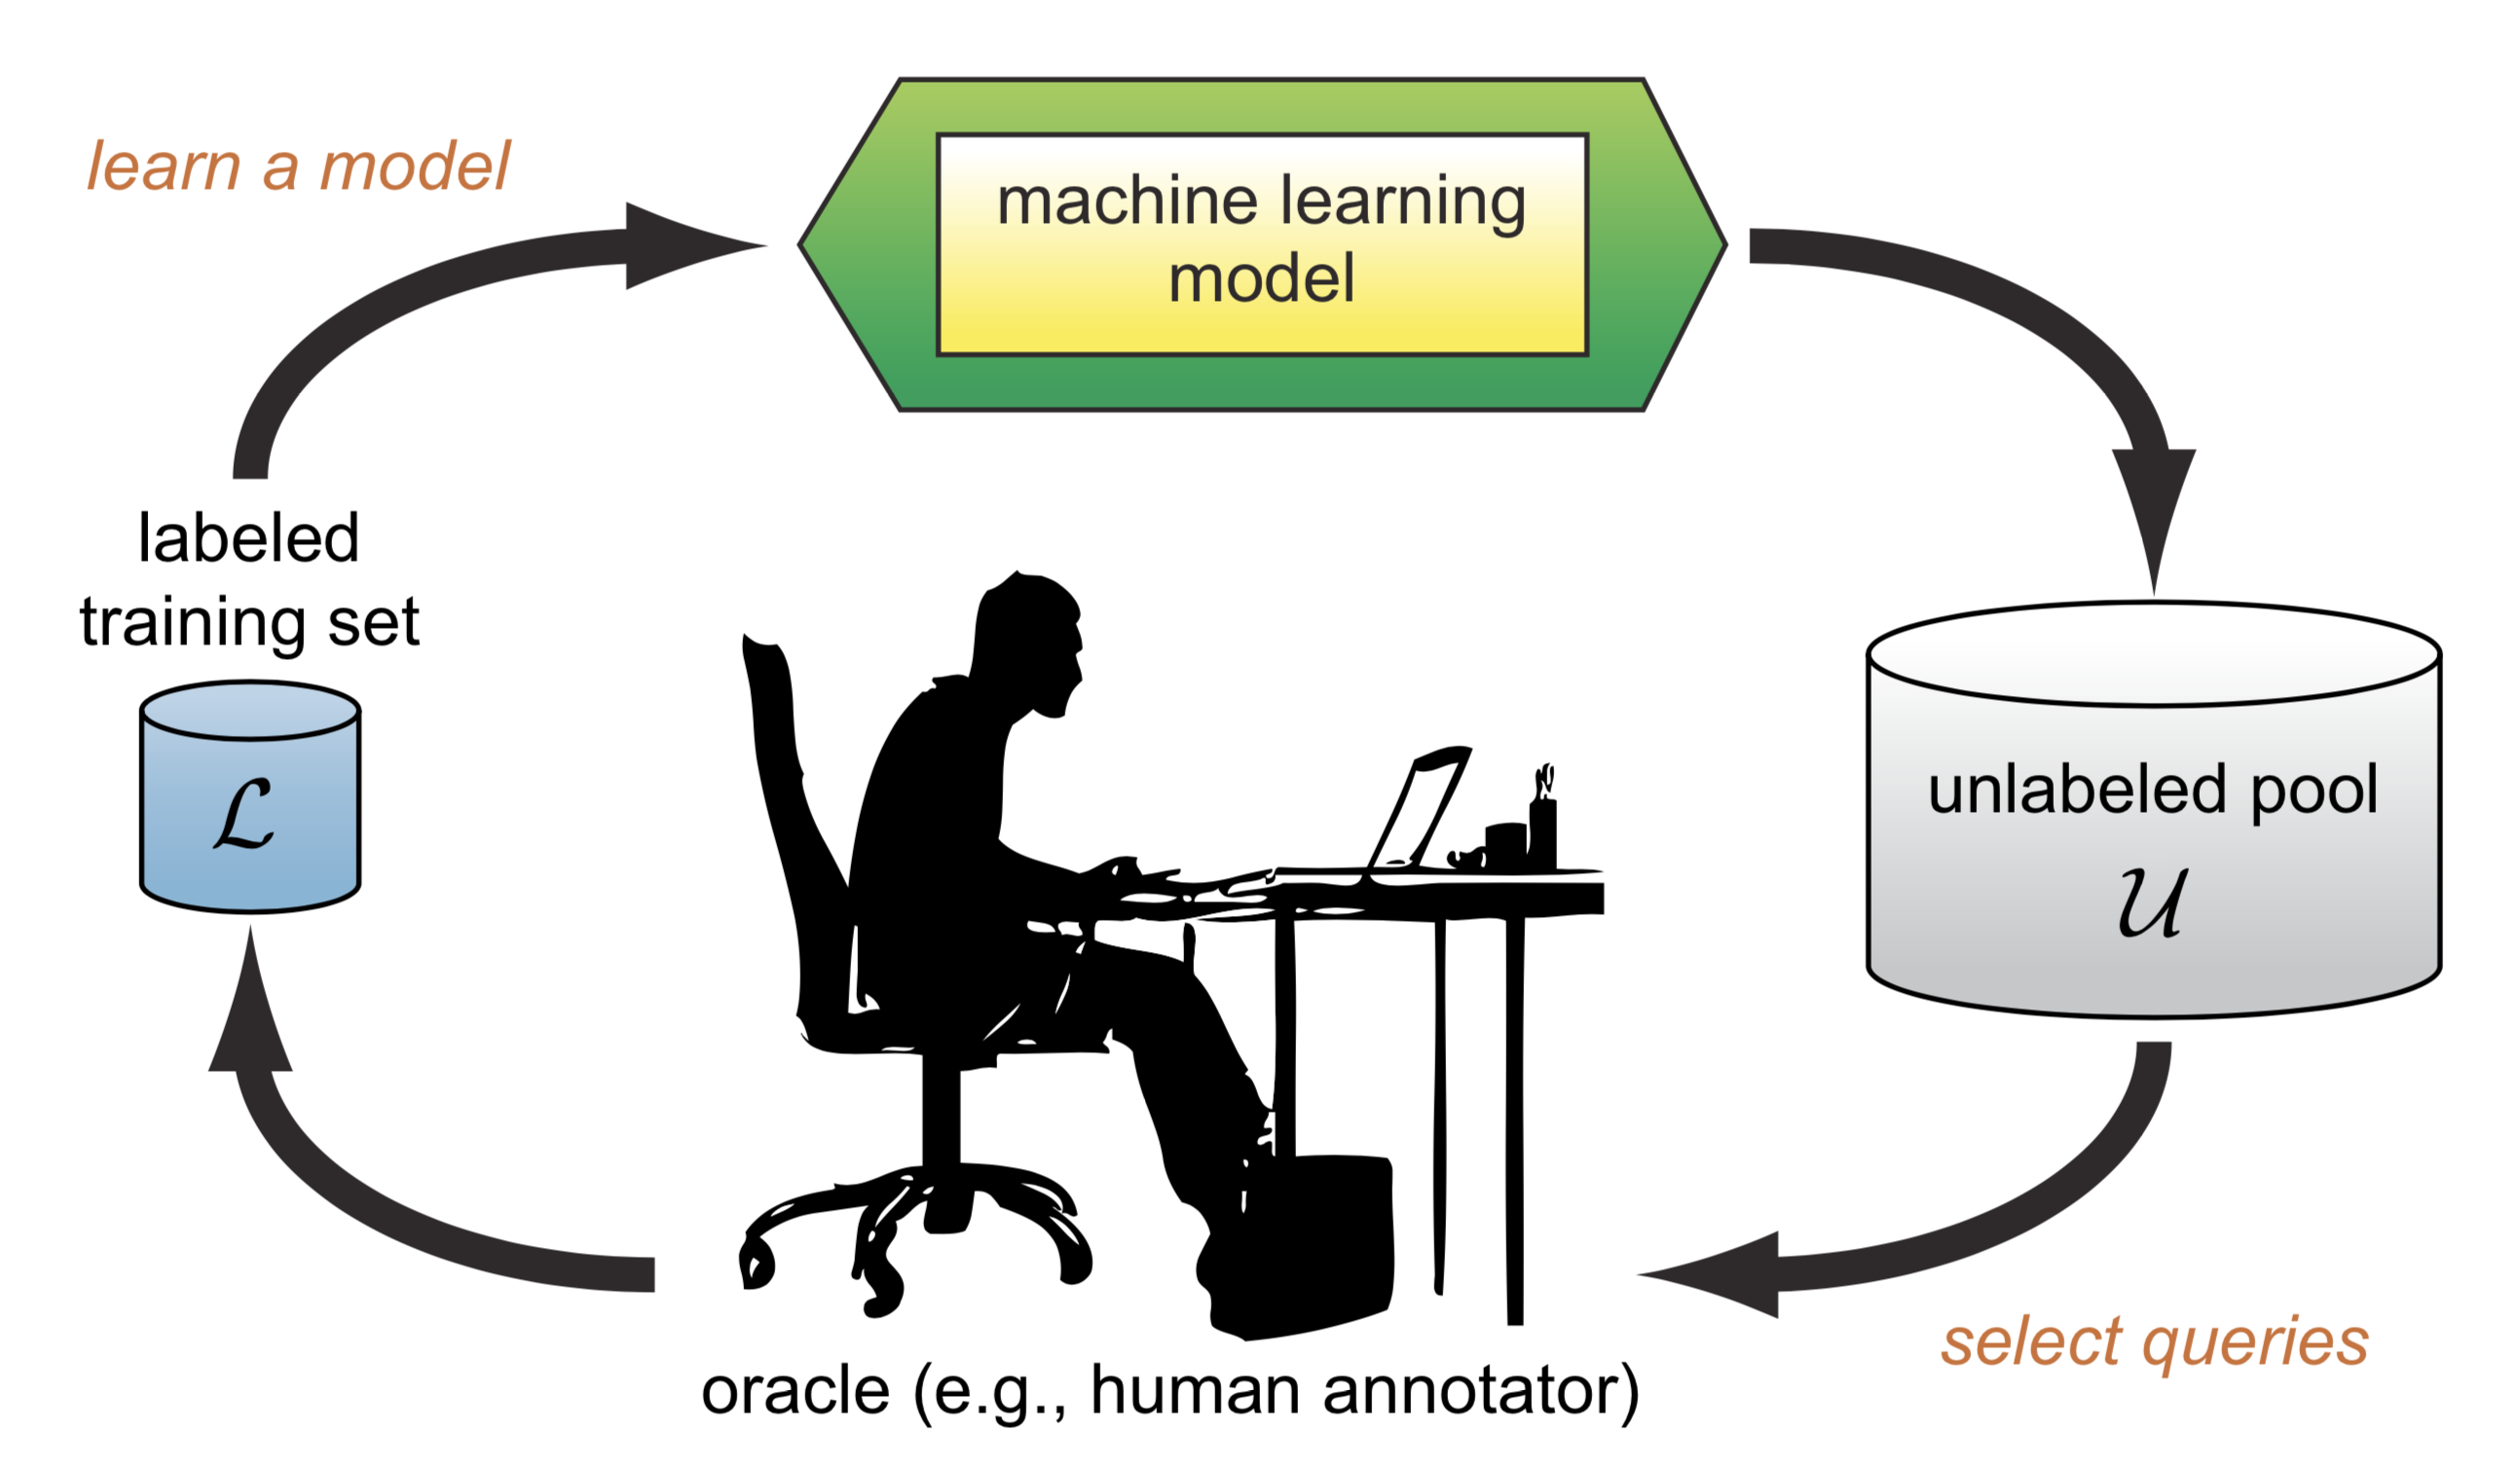
\includegraphics[width=1\linewidth]{ActiveLearningScheme.png}
\caption{Figure 1 from  \cite{settles2012active}, showing a typical ``pool-based active learning cycle''.}
\label{ActiveLearningExample}
\end{figure}

There are a variety of approaches to the active learning problem, however most involve the use of an \textit{acquisition function}, which selects which sample from $\mathcal{U}$ (the set of candidate unlabeled examples) should be selected for labeling and training \cite{settles2012active}. As the most appropriate training examples varies depending on the model itself, the chosen sample is said to be `queried' by the algorithm. One of the most common query methods is that of \textit{uncertainty sampling} \cite{settles2012active}, wherein the samples that the learning algorithm is most uncertain about labeling are queried. We will suggest in this paper that algorithm uncertainty can provide an effective measure of sample difficulty which can be used to automate the construction of learning curricula.

A common way of estimating model uncertainty is by analysing the distance to classification threshold of the model outputs; for example one method is to select the sample about which the model is least confident in predicting (taken from \cite{settles2012active}):
\begin{equation}
x^{*}_{LC} = \arg\max_{x} 1 - P_{\theta}(\hat{y}|x),
\end{equation}
where
\begin{equation}
\hat{y} = \arg\max_{y_i}P_{\theta}(oftsy_i|x).
\end{equation}
Where $x^{*}_{LC}$ is the queried training sample and $P_{\theta}(y_{i}|x)$ is the model's predicted probability that sample $x$ is of class $y_{i}$, given model parameters $\theta$. Similarly, samples can be queried by their average distance to classification threshold or, similarly, the entropy of the algorithm prediction, again taken from \cite{settles2012active}:
\begin{equation}
x^{*}_{H} = \arg\max_{x} - \sum_{i} P_{\theta}(y_i|x)\log P_{\theta}(y_i|x),
\end{equation}
where the sum runs over the possible classes $y_i$. More sophisticated methods for estimating prediction uncertainty include the ``Bayesian Active Learning by Disagreement (BALD)'' \cite{houlsby2011bayesian} acquisition function, which is used for deep models by the authors of \cite{gal2017deep} and is introduced and used in Chapter \ref{ch:DAC} of this paper.

It is interesting to note the somewhat opposing assumptions underlying active and curriculum learning; in the active learning approach the \textit{most} uncertain samples, which could arguably be seen as `hard' samples from a curriculum point of view, are selected for training. In curriculum learning however, the focus is usually on selecting easy samples, particularly early on in training, to improve model performance. Again, this speaks to the dynamic discussed in \cite{ELMAN199371}, where the author lays out potential justifications for the learning benefits of emphasizing both easy and hard/noisy training samples. As we will see in the results sections of Chapter \ref{ch:DAC}, our experiments support this idea, with both `easy to hard' and `hard to easy' curricula improving model performance in some cases

There are many examples of authors implementing active learning approaches for a variety of algorithms; \cite{tong2001support} develops various methods to query unlabeled samples using support vector machines to categorize news stories, while \cite{yang2003automatically} uses active learning to reduce the burden of human effort in labeling video data. In a more recent study, the authors of \cite{wang2017cost} employ active learning with deep networks for image classification, successfully reducing the number of training samples required to achieve promising results on challenging image classification tasks such as face recognition. Several  studies investigate theoretical justifications for the benefit of active learning and the situations in which it is beneficial to learning, for example \cite{balcan2006agnostic} and \cite{balcan2010true}. However in most cases these studies are based on severely restricted hypothesis spaces and more general proofs are yet to be developed \cite{settles2012active}. While the main goal of active learning is generally to reduce the number of samples required to achieve a certain level of test set performance \cite{settles2012active}, there are some studies that examine how active learning approaches can reduce overall generalization error, for example \cite{cohn1994improving}. This motivates the idea underlying this paper, that active learning methods can be used in a an automated curriculum learning setting in order to improve the overall accuracy of deep models. 

We have now introduced the main componentry that will be employed in the rest of the paper; specifically we will use methods motivated by uncertainty sampling in active learning to estimate training example difficulty scores which will be used to automatically construct learning curricula. In the following chapter we will outline several recent studies which have tested methods for automating the process of curriculum construction, before laying out the methods and experimental results carried out for this report in the subsequent two chapters. 

\chapter{Related Work}

\section{Self Paced Learning}

\section{Transfer Learning}

\section{Reinforcement Learning}

\section{Active Learning}

\chapter{Methods}

\section{Active Learning Metrics}
The purpose of this paper is investigate how different active learning query metrics can be used to automatically construct learning curricula to improve the generalization performance of deep models. As such we select several active learning approaches, each of which can be used in combination with a curriculum construction methodology (REF SECTION) during training. Testing several methods will also allow us to test the robustness of the results and ascertain whether or not performance differences are consistent across different methods. 

Each active learning method will be used to score the training samples, with the score then being fed as an input into the curriculum construction method to build the training mini-batches throughout the learning phase. As we are not `acquiring' samples, rather we are calculating a score for every training sample, the terminology `acquisition function' would be inappropriate, instead we refer to these score producing functions as \textit{active score functions}.  Each function will map training samples to a real number, which is then passed through a softmax function; this has the effect standardizing the various metrics, as well as allowing us to control the score ratio between different functions using the softmax temperature, as well as producing an output that can interpreted as sampling probabilities (see \ref{Methods_SoftmaxTemperature}). In order to have consistency across the different methods we invert certain scores so that a \textit{higher} score for a sample always corresponding to the sample being estimated to be \textit{easier} for the sample to classify. The classic curriculum learning approach would therefore bias learning towards samples with high scores, while the classic active learning approach would bias learning towards samples with low scores. 

As well as monitoring how the different active score functions affect model performance, we will also investigate how successful the different methods are at identifying which samples are `hard' or `easy', by visually inspecting the samples which receive very high or low scores by the different functions throughout training. 
\subsection{Average Absolute Distance to Threshold (AADT)}
As laid out in section \ref{Background_ActiveLearning}, a popular active learning method is to examine the proximity to the classification boundary of the model's outputted probabilities (assuming the model outputs probabilities; we will be using deep models with a softmax output layer). The assumption is that samples that the model is uncertain about classifying will produce probabilities close to the classification boundary; indeed as mentioned in section \ref{Background_ActiveLearning} the authors of REF show that prediction variance is inversely proportional to the distance to the boundary. From a curriculum perspective we can estimate a sample's difficulty by the algorithm's uncertainty in predicting the class label, with uncertain samples being seen as hard, and vice versa. 
We therefore calculate the distance to threshold active score function as follows, note that the score is proportional to the \textit{inverse} of the average distance to threshold, in order to ensure that easier samples have a higher score and vice versa:
\begin{equation}
P_{\theta}^{AADT} (x_i) = \frac{exp(\frac{S^{AADT}_{\theta}(x_i)}{\tau})}{\sum_{j}^{N} exp(\frac{S^{DT}_{\theta}(x_j)}{\tau})},
\end{equation}
where
\begin{equation}
S^{AADT}_{\theta}(x_i) = \frac{C}{ \sum_{c}^{C} \left|P_{\theta}(y_c |x_i) - \frac{1}{C}\right|}.
\end{equation}
Where $|.|$ represents the L1 norm/absolute value function.
Here $N$ is the number of training samples, $C$ is the number of output classes and $P_{\theta}(y_c |x_i)$ is the output softmax probability for class $y_c$ of the model parameterised by $\theta$, given input $x_i$. We tried a similar approach using the \textit{square} of the distance to threshold, as opposed to the absolute distance to threshold however results were extremely similar. 

\subsection{Classification Entropy (H)}
Again, as laid in section \ref{Background_ActiveLearning}, a popular uncertainty measure is the entropy of the probabilistic model output. Here, samples which produce outputs with higher entropy represent samples that the model is uncertain about classifying, or, from the curriculum perspective, we see as being `hard' samples. The classification entropy active score function is calculated as follows:

\begin{equation}
P_{\theta}^{H} (x_i) = \frac{exp(\frac{S^{H}_{\theta}(x_i)}{\tau})}{\sum_{j}^{N} exp(\frac{S^{H}_{\theta}(x_j)}{\tau})},
\end{equation}
where
\begin{equation}
S^{H}_{\theta}(x_i) = - \sum_{c}^{C} P_{\theta}(y_c|x)\log P_{\theta}(y_c|x).
\end{equation}

\subsection{BALD}
Recent advances in Bayesian neural networks and variational inference motivate an alternative approach to measuring uncertainty; while the distance to classification threshold may encapsulate classification uncertainty for samples close to the boundary, it does not consider the uncertainty associated with analysing samples from parts of the feature space that is not represented in the training data. Consider the toy example shown in FIGURE, where a sample may be far from the classification boundary, but so dissimilar from the training samples that we would want to measure the sample as having high classification uncertainty. One approach to this problem is given by REF GAL, where they motivate using the \textit{Monte Carlo dropout} method as a way of approximating variational inference in neural networks. As with the usual dropout procedure, weights are randomly set to zero throughout the training phase, however, unlike the usual approach, dropout is maintained at the test stage, and a number of forward passes are carried out, resulting in a distribution of outputs. The resultant distribution can subsequently be analysed to infer which test samples the model is more or less confident in predicting, for example by comparing the variance of the output distributions. In REF GAL ACTIVE LEARNING, the authors use the MC dropout method to construct an active learning acquisition function \textit{Bayesian Active Learning by Disagreement (BALD)}, which queries points which ``maximise the mutual information between predictions and model posterior'', identifying samples that have a high probability of being placed into different classes in the different stochastic forward passes. One interpration of the BALD method is that it is similar to the `Query by Committee'' active learning methods, with the different forward passes representing different models' votes. 

We calculate the BALD active score function as follows:

\begin{equation}
P_{\theta}^{BALD} (x_i) = \frac{exp(\frac{S^{BALD}_{\theta}(x_i)}{\tau})}{\sum_{j}^{N} exp(\frac{S^{BALD}_{\theta}(x_j)}{\tau})},
\end{equation}
where
\begin{equation}
S^{BALD}_{\theta}(x_i) = - \sum_{c}^{C} \bar{P}_{\theta}(y_c|x_i)\log( \bar{P}_{\theta}(y_c|x_i)) + \frac{1}{M} \sum_{m}^{M} (\sum_{c}^{C} P^{m}_{\theta}(y_c|x)\log(P^{m}_{\theta}(y_c|x))),
\end{equation}
and
\begin{equation}
 \bar{P}_{\theta}(y_c|x_i) = \frac{\sum_{m}^{M}P^{m}_{\theta}(y_c|x)}{M}. 
\end{equation}
Here $M$ is the number of stochastic forward passes carried out and $P^{m}_{\theta}(y_c|x)$ is the softmax probability of class $c$ from the $m^{th}$ forward pass. The score can therefore be interpreted as the difference between the entropy of the average softmax output and the average entropy of the output of each forward pass.
\subsection{Softmax temperature}\label{Methods_SoftmaxTemperature}
In order to homogenize the outputs of the different active score functions, we pass the the scores through a softmax functions, resulting in an output of softmax probabilities summing to 1. Using the softmax function also allows us to use the softmax temperature in order to control the diversity of the sampling probabilities. A common issue with active learning is that the acquisition functions can end up sampling from an unrepresentative subset of the input space, resulting in significant bias in the training of the model (REF!). Indeed, GIVE EXAMPLE OF MAX RATIO FOR DIST2THRESH

We control this effect by using the softmax temperature to target a preset \textit{maximum probability ratio}, defined as follows:
\begin{equation}
Max Ratio = \frac{\max_{i} P_\theta(x_i)}{\min_{i} P_\theta(x_i)}.
\end{equation}
To do this we begin with a softmax temperature of 1, then calculate the current maximum probability ratio and increment the temperature until the target ratio is achieved. Pseudocode is given below:

PSEUDOCODE FOR SOFTMAX CONTROL

The downside to this method is it could be skewed by outlier probabilities; if there were one sample with an extremely large sampling probability this method would still achieve a target maximum probability ratio, without achieving sufficient diversity in the sampling probabilities. We investigated using winsorization (REF) as an outlier removal technique prior to tuning the temperature parameter, however, as the active score functions we use generally did not result in outliers, this did not affect results.  We show in section REF how controlling the maximum probability ratio affects training. 

\section{Curriculum Construction}

\subsection{Biased Sampling}

\subsection{Uniform Sampled Tasks}
Similar to self-paced learning
\subsection{Biased Sampled Tasks}


\section{Datasets}
Description, example, dataset size, source
\subsection{MNIST}

\subsection{Geometric Shapes}

\subsection{CIFAR 10}

\section{Architectures}

\chapter{Bootstrapped Active Curricula}\label{ch:BootstrappedActiveCurricula}
The first curriculum construction approach we investigate is what we term \textit{bootstrapped active curricula (BAC)}, the name is chosen as it involves `bootstrapping' a curriculum from a separate model. The intuition behind this approach is that, while it may be difficult to ascertain a-priori which samples are `hard' or `easy' (particularly for very large datasets where it is infeasible to analyse every sample), we can automatically infer which samples are difficult by first training a model on the data and then using an active learning uncertainty metric to investigate which samples the model is uncertain about classifying. Using prediction uncertainty to approximate difficulty, we can then construct a learning curriculum which can be used to train a new model, for example by splitting the training samples into separate tasks of increasing difficulty, as detailed below.
\section{Curriculum Construction}
In the BAC approach we train two models; the first, which we term the `baseline model' and denote  $\theta_{baseline}$, is trained to convergence using a standard mini-batch gradient descent optimisation on the entire available training set $\mathcal{T}$. We then use $\theta_{baseline}$ in conjunction with the Absolute Average Distance to Threshold uncertainty function as defined below in Section \ref{BAC_AADT}, scoring each training sample in $\mathcal{T}$. This produces $\mathbf{s}^{\theta_{baseline}}$, a vector of $N$ scores, where $N$ is the number of samples in $\mathcal{T}$, such that the $i^{th}$ element of $\mathbf{s}^{\theta_{baseline}}$ is the output of the AADT uncertainty function for the $i^{th}$ training sample inputs:

\begin{equation}\label{eq:BAC_S}
s^{\theta_{baseline}}_i = AADT_{\theta_{baseline}}(x_i) 
\end{equation}
where $x_i$ are the inputs of the $i^{th}$ training sample. We then abuse the function notation slightly to set $\mathbf{s}^{\theta_{baseline}} = AADT_{\theta_{baseline}}(\mathcal{T}) $, i.e. signifying that $\mathbf{s}^{\theta_{baseline}} $ is the output of the AADT uncertainty function over the entire training set $\mathcal{T}$.

 We then sort the training samples according to their score, producing an ordered training set $\mathcal{T}_{\mathbf{s}^{\theta_{baseline}}}$, such that the first training sample in $\mathcal{T}_{\mathbf{s}^{\theta_{baseline}}}$ is the sample which produces the highest value from the AADT function. We then split $\mathcal{T}_{\mathbf{s}^{\theta_{baseline}}}$ into equally sized `tasks', with the number of tasks being a hyperparameter of the curriculum construction. The learning curriculum is then constructed from these tasks; the chosen approach is to split training into discrete phases, with the number of phases being equal to the chosen number of tasks. The first phase of the curriculum consists of training only on the first task, denoted $\mathcal{T}^1_{\mathbf{s}^{\theta_{baseline}}}$, in the second phase, the second task is added to the training samples, training the model on $\mathcal{T}^1_{\mathbf{s}^{\theta_{baseline}}}\cup\mathcal{T}^2_{\mathbf{S}^{\theta_{baseline}}}$. In the third phase (if the number of tasks is greater than 2), the next task is added, and so on until all tasks have been added and the final phase consist of training on the entirety of the original training set $\mathcal{T}$. Having constructed the BAC learning curriculum, we train a new `curriculum' model', which we denote by $\theta_{curriculum}$, using the curriculum. Pseudocode for the BAC method is given in Section \ref{BACPseudocode}.

\subsection{Average Absolute Distance to Threshold (AADT)}\label{BAC_AADT}
A popular active learning uncertainty method is to examine the proximity of the model's outputs to the classification boundary. The assumption is that samples that the model is uncertain about classifying will produce probabilities close to the classification boundary; indeed as mentioned in Section \ref{Background_ActiveLearning} the authors of \cite{Chang18} show that prediction variance is inversely proportional to the distance to the boundary. From a curriculum perspective we can estimate a sample's difficulty by the algorithm's uncertainty in predicting the class label, with uncertain samples being seen as hard, and vice versa. We thus define the uncertainty function $AADT$ which calculates the absolute distance to classification threshold for the model outputs, averaged across all possible classes. Note that the function is dependent on a the output of the model in question, which is denoted $\theta$.
\begin{equation}
AADT_{\theta}(x_i) = \frac{ \sum_{c=1}^{C} \left|P_{\theta}(y_c |x_i) - \frac{1}{C}\right|}{C}.
\end{equation}
Where $|.|$ represents the L1 norm/absolute value function.
Here $N$ is the number of training samples, $C$ is the number of output classes and $P_{\theta}(y_c |x_i)$ is the output softmax probability for class $y_c$ of the model $\theta$, given input $x_i$. We also tested the average \textit{square} of the distance to threshold, as opposed to the absolute distance to threshold, as well as testing the entropy of the outputs as an uncertainty measure, however results were extremely similar in all cases.

\subsection{Phase Training Epochs}
A naive approach to the BAC approach would be to train the curriculum model for the same number of epochs as the baseline model, split equally across training phases. For example if the baseline model was trained for 100 epochs and we then constructed a two task curriculum, the curriculum model would be trained on the first task for the first 50 epochs, then on both tasks for the second 50 epochs. The issue with this method however is that, as during the first 50 epochs there are only half as many training samples, the curriculum model will not have as many parameter updates as the baseline model. To emphasize this, consider that if we were using stochastic gradient descent (i.e. a mini-batch size of 1) with a full training set of 1000 samples, the baseline model in this instance would have (\# epochs * \# training samples) parameter updates, i.e. 100 * 1000 = 100,000 parameter updates. The curriculum model on the other hand would have (50*500) parameter updates the first training phase and (50*1000) in the second, resulting in a total of   (50*500) + (50*1000) = 75,000 parameter updates, 25\% less updates than the baseline model. To address this, we increase the number of epochs in each phase by the ratio of the number of samples used in the phase to the size of the whole training set. Specifically, we set the number of training epochs in each phase as follows:
\begin{equation}\label{eq:BAC_Epochs}
NumEpochs^{t} =\floor{ \frac{BaselineEpochs}{t}}
\end{equation}
Where $BaselineEpochs$ is the number of epochs used to train the baseline model and $NumEpochs^{t}$ denotes the number of training epochs in the $t^{th}$ training phase. For example, in the first phase, $NumEpochs^{1} = \frac{BaselineEpochs}{1} = BaselineEpochs$. $\floor{.}$ represents the floor function; as $\frac{BaselineEpochs}{i}$ will not always be integer, we round down the number of epochs in each phase. The curriculum model will therefore be trained for a higher number of epochs (precisely, $\sum_{t=1}^{NumTasks}{\frac{1}{t}}$ times more epochs), however the number of parameter updates will be equalised. 

\subsection{Pseudocode for BAC}\label{BACPseudocode}
Pseudocode for the boostrapped active curriculum method (assuming the use of the AADT uncertainty function and an easy to hard curriculum):
\begin{algorithmic}
\FOR {$Num\_Epochs$}
\STATE $\text{train }  \theta_{baseline} \text{ on training set } \mathcal{T}$
\ENDFOR
\STATE $\mathbf{s}^{\theta_{baseline}} = AADT_{\theta_{baseline}}(\mathcal{T})$
\STATE $\mathcal{T}_{\mathbf{s}^{\theta_{baseline}}} = \mathcal{T}, \text{sorted by } \mathbf{s}^{\theta_{baseline}} \text{ (descending order)}$ 
\STATE $Num\_Samples = |\mathcal{T}_{\mathbf{s}^{\theta_{baseline}}}|$
\FOR {$t=0$ to $Num\_Tasks$}
\STATE $TaskStartIndex = Num\_Samples*\frac{t}{Num\_Tasks} $
\STATE $TaskEndIndex = Num\_Samples*\frac{t+1}{Num\_Tasks} $
\STATE $\mathcal{T}^{t}_{\mathbf{s}^{\theta_{baseline}}} = \mathcal{T}_{\mathbf{s}^{\theta_{baseline}}}[TaskStartIndex:TaskEndIndex,:] $
\ENDFOR
\FOR {$t=0$ to $Num\_Tasks$}
\STATE $Num\_Epochs\_Task = \floor{\frac{Num\_Epochs}{t}}$
\FOR{$Num\_Epochs\_Task$}
\STATE $\text{train }  \theta_{curriculum} \text{ on training set } \mathcal{T}^{0:t}_{\mathbf{s}^{\theta_{baseline}}} $
\ENDFOR
\ENDFOR
\end{algorithmic}

\section{Geometric Shapes Dataset}\label{sec:GeoShapes}
To test the boostrapped active curriculum approach we use the `Geometric Shapes' dataset \cite{GeoShapes}, as used in \cite{Bengio2009}. This dataset consists of 32x32 pixel images of geometric shapes, specifically ellipses, rectangles and triangles; the class labels are one-hot vectors which indicate to which of the three classes each sample belongs. As well as varying the shapes shown in the image, the samples also vary in colour, orientation, size and position. This dataset is used in \cite{Bengio2009} as it is easy to construct a predefined curriculum for geometric shapes; circles, squares and equilateral triangles represent regular, `easy' versions of the broader classes of ellipses, rectangles and triangles, respectively. The authors of \cite{Bengio2009} train a curriculum model by first training only on an easy training set consisting only of circles, squares and equilateral triangles, before then training on a hard training set with the more general shapes. The easy and difficult training sets consist of 10,000 training samples, giving a total of 20,000 training samples, while the test set, consisting only of hard samples, contains 5,000 images. The authors demonstrate that their approach outperforms an identical model trained only on the harder shapes; the curriculum model consistently achieves greater test accuracy, with the greatest improvement coming  when the first half of the training epochs train on the easier shapes, and the second half the harder ones, as shown in Figure 3 of their paper. As discussed by the authors, one potential pitfall of their experiments is that the curriculum model has seen more samples than the benchmark model, as it has been trained on both the easy and the difficult training sets, to avoid this in our experiments, the training set we use is the union of both the easy and difficult samples. Our training set therefore consists of 20,000 geometric shape images, including both the easy, regular shapes and the more difficult shapes, the test set is unchanged however, consisting of the 5,000 difficult samples. 

Some example images for the Geometric Shapes dataset are given in Figure \ref{fig:GeoSamples} below, with Figure \ref{fig:EasyGeoSamples} showing examples from the easy training set featuring circles, squares and equilateral triangles, while Figure \ref{fig:HardGeoSamples} shows samples from the more difficult training set of general shapes.

\begin{figure}
\hspace*{-2cm}    
\centering
\begin{subfigure}{.6\textwidth}
  \centering
  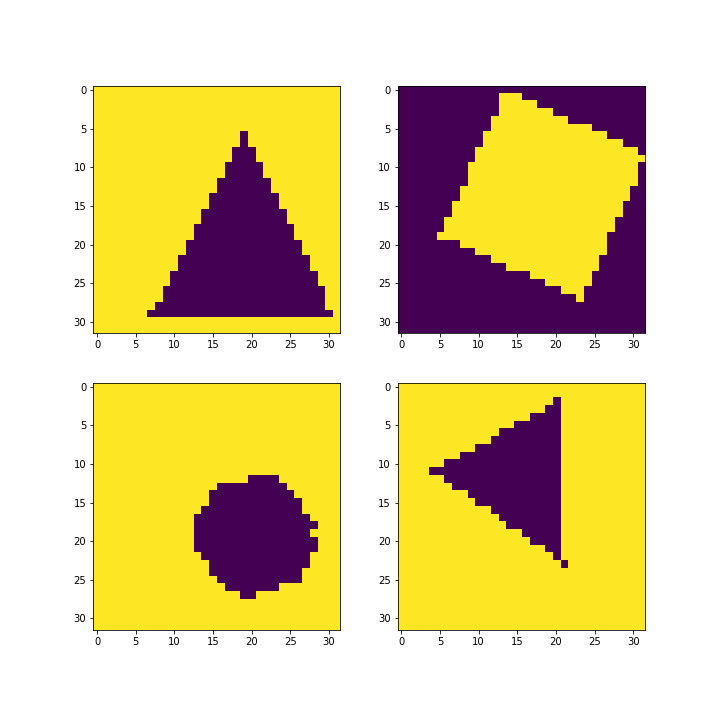
\includegraphics[width=1\linewidth]{EasyGeoShapesExamples.png}
  \caption{Samples from `easy' training set}
  \label{fig:EasyGeoSamples}
\end{subfigure}%
\begin{subfigure}{.6\textwidth}
  \centering
  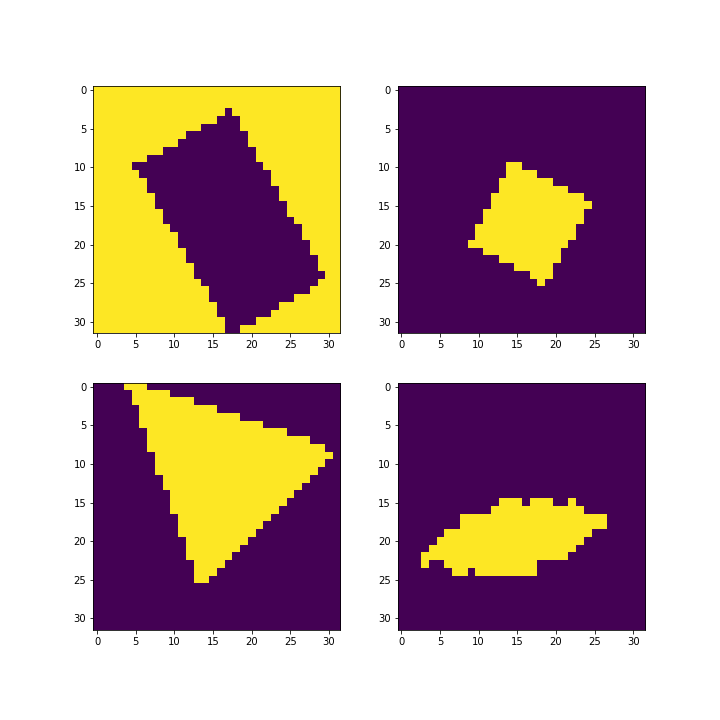
\includegraphics[width=1\linewidth]{HardGeoShapesExamples.png}
  \caption{Samples from `hard' training set}
  \label{fig:HardGeoSamples}
\end{subfigure}
\caption{Sample figures from the Geometric Shapes dataset}
\label{fig:GeoSamples}
\end{figure}

 In the results Section \ref{sec:BAC_Results}, we analyse how successful our tested curriculum method is at automatically identifying which samples come from the easy or hard training sets, investigating which training samples fall into the different tasks automatically constructed through the BAC curriculum method. 

\section{Experiments}
 In order to measure the effect of the curriculum on test performance, we set $\theta_{baseline}$ and $\theta_{curriculum}$ to have identical architectures, hyperparameters and initial weights, essentially minimizing any differences in training besides the learning curriculum. We use both the Average Absolute Distance to Threshold (AADT) function, detailed in Section \ref{BAC_AADT}, to score the training samples with the trained baseline model in each experiment. Furthermore, as well as testing `easy to hard' curricula, where the training phases progress from  $\mathcal{T}^1_{\mathbf{s}^{\theta_{baseline}}}$ to the final task, we also test the opposite approach, with the first training phase using only the hardest task, then incorporating the other, easier tasks throughout training. We run the experiments using the Geometric Shapes dataset, as introduced in Section \ref{sec:GeoShapes}, allowing us to compare results with the predefined curriculum as in \cite{Bengio2009}. To do so, as well as training the baseline and BAC curriculum models, we also train a model using the predefined curriculum method laid out in \cite{Bengio2009}, specifically training on only the easy samples in for the first half of the training epochs, and only the hard samples in the second half. In order to better compare the predefined curriculum method from \cite{Bengio2009}, we also run an adjusted version of their method; unlike the BAC approach, where we correct the difference in number of parameter updates between the curriculum model and the baseline model, the predefined curriculum model will end up undergoing significantly less parameter updates than our baseline (in fact it will have half as many updates). We therefore correct for this in two ways; in the first phase of training, in which the model is trained only on the easy images, lasts for twice as many epochs as in the unadjusted method (correcting for the fact that it consists of half as many samples as the full training set). The second phase of the adjusted model is then trained on the \textit{full} training set, consisting of the union of the hard and easy samples. This should allow for a better comparison between the BAC models, the baseline model, and the predefined curriculum approach. We therefore train 5 separate models:
 \begin{itemize}
 \item Baseline Model - Trained on the full training set of easy and hard geometric shape images for all epochs, with standard mini-batch stochastic gradient descent.
 \item Easy to Hard Model - Trained with a boostrapped active curriculum construct from the above Baseline Model, beginning with the easiest/least uncertain task and including the other tasks throughout training.
 \item Hard to Easy Model - As above, but training begins with the hardest/most uncertain tasks before incorporating the easier tasks throughout training.
 \item Predefined Curriculum - As in \cite{Bengio2009}, the first half of the training epochs use only the 10,000 easy training samples, while the second half train on only the 10,000 hard training samples.
 \item Adjusted Predefined Curriculum - As above, but the number of epochs in the first phase of training is doubled to account for the difference in parameter updates, and the second phase uses both easy and hard training samples for better comparison with the BAC models.
 \end{itemize}
 
All models are tested on the same test set of 5000 images, all containing `hard' geometric shapes; experiments are repeated multiple times with different weight initialisations. To analyse the effect of the curriculum on learning we report the accuracy and cross-entropy error of the different models over the held out test set. The exact model architecture is given in tables 5.1 - 5.3 below (`FC' = fully connected Layer):
 
\begin{table}[h]
\caption{Geometric Shapes Dataset Model Architecture} \label{tab:GeoArchitecture}
\begin{tabular}{|c||c|c|c|c|c|c|c|}
\hline
\multicolumn{8}{|c|}{Geometric Shapes Dataset Model Architecture} \\
\hline
 & Layer 1 & Layer 2 & Layer 3& Layer 4 &Layer 5 & Layer 6 & Layer 7 \\
\hline
Layer Type & FC & Dropout & FC & Dropout & FC & Dropout  & FC \\
\hline
Units & 300 & NA & 300 & NA & 300 & NA & 3 \\
\hline
Activation & Tanh \footnotemark & NA & Tanh & NA & Tanh & NA & Softmax \\
\hline
\end{tabular}
\end{table}
\footnotetext{The Hyperbolic Tangent activation is chosen as this was this the activation used in \cite{Bengio2009}.}
We also lay out the hyperparameters for the training procedures in table \ref{tab:HyperParams} below, experiments were carried out in Keras \cite{chollet2015keras} with the Adam optimiser implemented with the default hyperparameters (except for the learning rate which is given in Table \ref{tab:HyperParams}):

\begin{table}[h]
\caption{Experiment Hyperparameters} \label{tab:HyperParams}
\begin{tabular}{|c||c|c|c|c|c|c|}
\hline
\multicolumn{7}{|c|}{Experiment Hyperparameters} \\
\hline
 &Epochs & Optimiser &Learning Rate & Dropout \% & Batch Size & Num Tasks \\
\hline
GeoShapes & 350 & Adam & 0.0001 & 0.25 & 32 & 2  \\
\hline
\end{tabular}
\end{table}


Architectures and hyperparameters were chosen and tuned in order to deliver a good level of performance without prohibitive training times, robustness tests were however carried out varying the model architectures and hyperparameters resulting in little change in the relative performance of the different methods. 
\section{Results and Discussion}\label{sec:BAC_Results}
The results of running the bootstrapped active curriculum experiments with the Geometric Shapes dataset are summarised Figure \ref{fig:GeoShapesBACResults} which shows the test set accuracies and cross entropy errors, including standard errors, derived from 24 experiments with different initialisations, full results are given in Table \ref{tab:GeoShapes BACResults}.

\begin{figure}[h]
\hspace*{-3cm}    
\centering
\begin{subfigure}{0.7\textwidth}
  \centering
  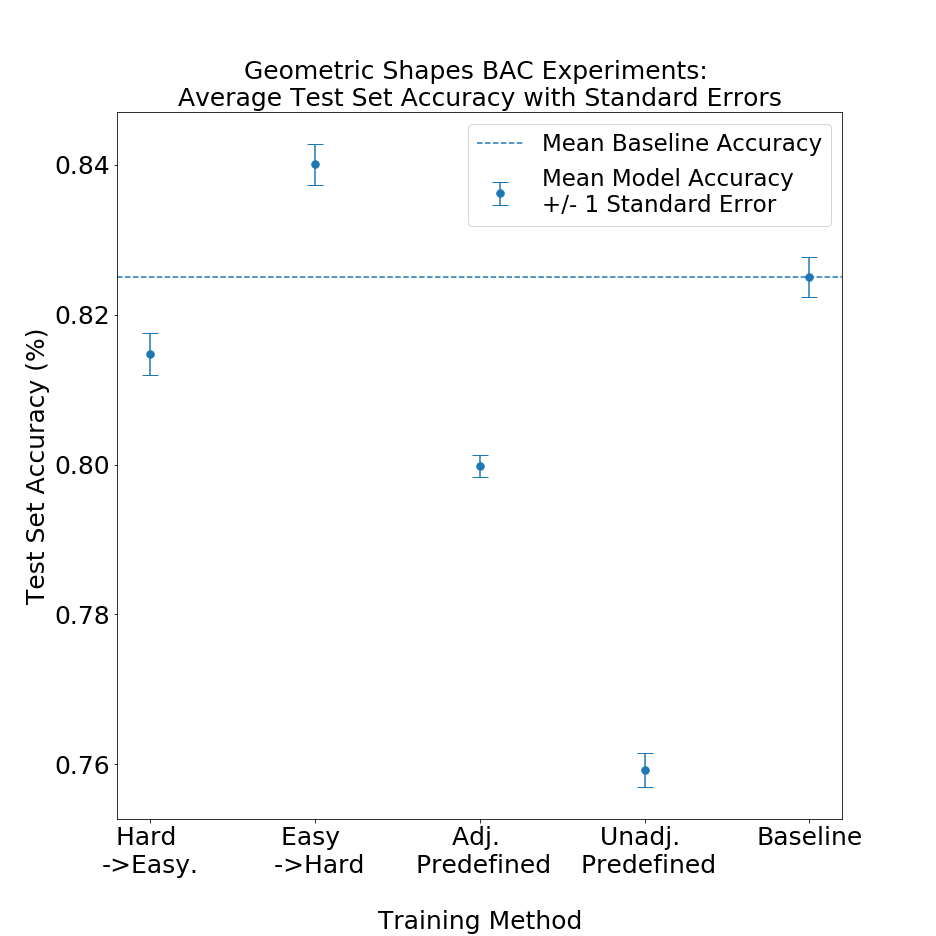
\includegraphics[width=1\linewidth]{GeoShapesBACResults_STE.png}
  \caption{ Mean Test Set Accuracies}
  \label{fig:BAC_StE}
\end{subfigure}%
\begin{subfigure}{0.7\textwidth}
\hspace*{-1cm}   
  \centering
  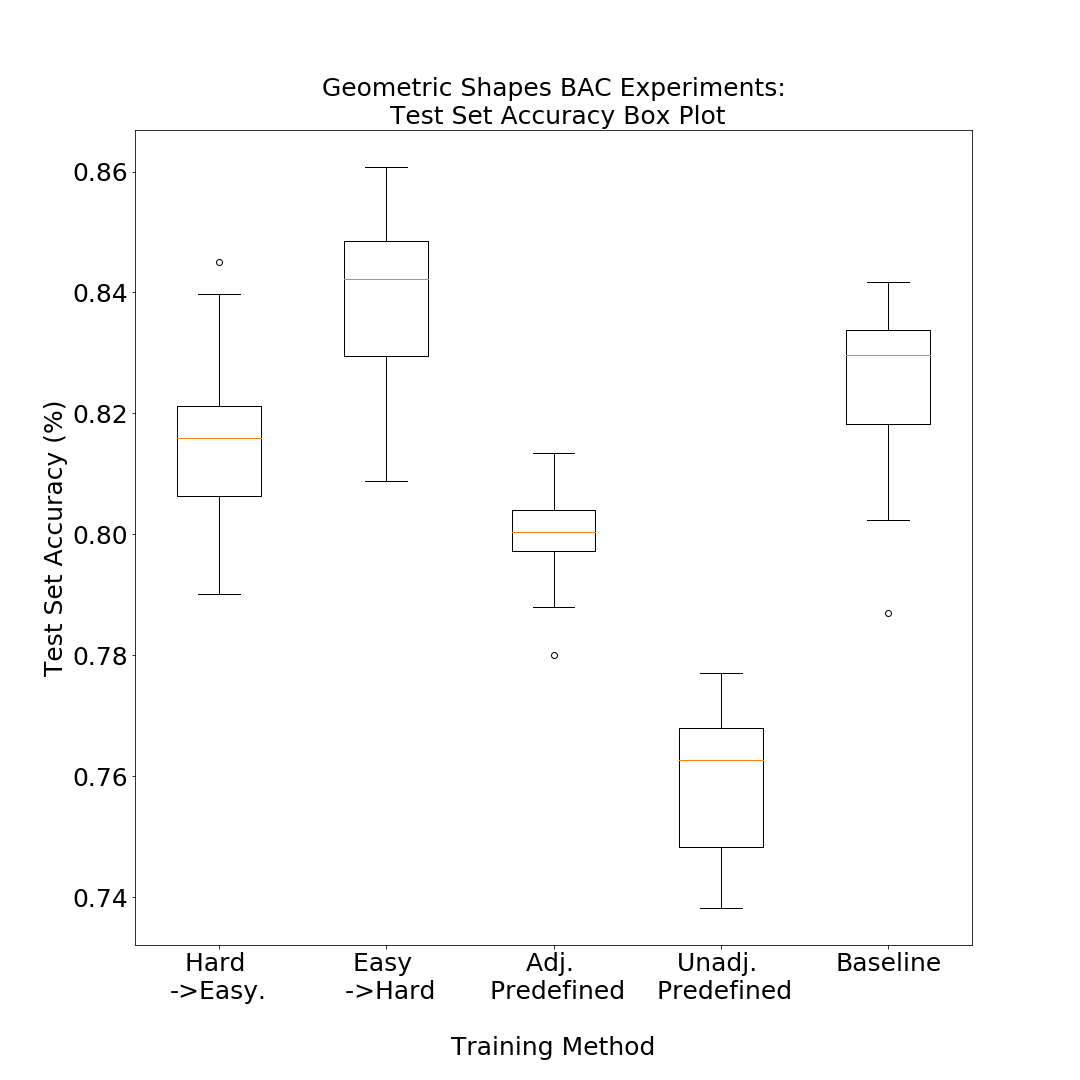
\includegraphics[width=1\linewidth]{GeoShapesBACResults_Boxplt.png}
  \caption{Test Set Accuracy Boxplots}
  \label{fig:BAC_Boxplt}
\end{subfigure}
\caption{Geometric Shapes Bootstrapped Active Curriculum (BAC) Experiment Results}
\label{fig:GeoShapesBACResults}
\end{figure}

We see from the results that the Easy to Hard curriculum model significantly outperforms the baseline model, with an average test accuracy improvement of around 2.5\%, over 5 standard errors, higher than the baseline test performance.  Cross-entropy error is also reduced, with the Easy to Hard curriculum test error over 6 standard errors below that of the baseline model. These results suggest that, not only is there a benefit to training the model with a curriculum, the BAC model seems to be successful at identifying which samples should be used in the different curriculum learning phases. Conversely, the other curriculum methods all underperform the baseline model; the Hard to Easy curriculum in some ways acts as a control, showing that the improvement in the Easy to Hard model is driven by the order in which the tasks are included in training, as opposed to being a consequence of another part of the BAC method. It is interesting to note that both of the predefined curriculum models underperform the baseline model; the lower accuracy of the unadjusted method would seem to support the authors' suggestion in  \cite{Bengio2009} that the performance differences in their experiments may have been a result of their curriculum model having seen overall more training samples than their baseline. However, even our adjusted version of the predefined curriculum results in a significantly lower test accuracy than the baseline. This is interesting as this method is effectively trained in the same way as the BAC approach, however the tasks are predetermined by an intuitive sense of difficulty, as opposed to being derived from the baseline. This would suggest that, even for datasets where there as a somewhat clear distinction between hard and easy samples, a bootstrapped curriculum may be more useful. Potentially, this may because the BAC method specifically calculates which samples the model itself is uncertain in classifying, as opposed to assuming that our intuitive sense of difficulty corresponds to the best curriculum for the model. We would note however, that given the relatively low resolution of the images (as illustrated in Figure \ref{fig:GeoSamples}), there is perhaps less observable difference between the easy and hard training sets than might be assumed, and that this may contribute to the poor performance of the predefined curriculum. Note that as we use a different baseline, these results are consistent with those shown in \cite{Bengio2009}; the baseline used in the referenced paper is trained only on the hard training set, whereas our baseline is trained on both the easy and hard training sets. In fact, in early experiments we tested using the same baseline as in \cite{Bengio2009} and found results consistent with the paper, with what we have termed the 'predefined curriculum' outperforming this more simple baseline.

With that in mind, we can analyse one of the the Easy to Hard curriculum experiments in more depth, in order to ascertain which samples are included in the two tasks. Recall that in the BAC method we train a baseline model, then use the uncertainty in the model's output class probabilities for the training samples, calculated using the AADT function defined in Section\ref{BAC_AADT}, to score and rank the training samples. The training samples are then split into two tasks, the first consisting of the training samples that the model is least uncertain in classifying, and the second task containing the samples about which the model's outputs are most uncertain. We can analyse the composition of the two tasks to infer which samples the model is least/most uncertain about. Doing so for one of the experiments presents some interesting conclusions; first of all, there is a significant lack of balance in the target classes in the two tasks. In task 1, the easier task, 43\% of the images are of triangles, while 31\% are of ellipses and 26\% are of rectangles, implying that the baseline model is significantly more confident in classifying whether or not an image shows a triangle than it is in classifying the other shapes. The bottom right image in Figure \ref{fig:HardGeoSamples} illustrates why this may be, with an example of an ellipse that looks quite similar to a mis-shapen rectangle, again this is probably the result of the low resolution of the images. We also observe that 64\% of the samples in the first task are from the easy training set of squares, circles and equilateral triangles, showing that the AADT function is somewhat successful in separating the two training sets, however the first task still contains a substantial number of the harder samples.

A potential enhancement to the BAC method would be to control the balance of the classes in either task, however if one class is indeed easier than the others to classify then it may be better for it to be over-represented in the easier task(s). While we used two tasks for the Geometric Shapes dataset as this corresponded to the number of tasks of the predefined curriculum, we also ran some initial experiments with a larger number of tasks. We found some variation in results with a larger number of tasks, with some choices of task number underperforming the baseline model, however further tests could be carried out in future work to ascertain how robust these results are and investigate what is driving the different performances.
\section{Summary}
To summarize, these experiments seem to support the hypothesis that training a deep model with a curriculum can reduce generalization error, and furthermore that using an active learning approach to inferring sample difficulty through model prediction uncertainty can be an effective way of automatically constructing such curricula. In particular such curriculum construction methods may even outperform a preconstructed curriculum using an intuitive sense of sample difficulty, as model uncertainty incorporates information about which samples the model itself finds difficult. One of the arguable drawbacks to the BAC method is that it requires that a baseline model is trained to convergence, in order to use its outputs to construct the curriculum to train the curriculum model. This effectively doubles the training time and, while this may not be too significant a computational burden in some problems, motivates the approach of the next chapter, which investigates whether or not a curriculum can be constructed dynamically throughout training, without first training a baseline model.





\chapter{Dynamic Active Curricula}
The results laid out in Chapter \ref{ch:BootstrappedActiveCurricula} suggest that generalisation performance can indeed be improved through the use of a learning curriculum, and that using active learning approaches to score which training samples are hard or difficult can be an effective way of automatically constructing such curricula without manually analysing the training samples. The disadvantage with the BAC method from Chapter \ref{ch:BootstrappedActiveCurricula} however is that it is necessary to first train a `baseline' model that can be used to derive a curriculum based on which samples it is uncertain about classifying. While in some cases this may not too significant a computational burden, it does effectively double the overall training time, motivating the approach laid out in this section. Specifically, we wish to investigate methods that can dynamically construct a curriculum throughout training, without needed to reference another model. We do this by calculating the model uncertainty on the training samples throughout training, using the uncertainty scores to construct dynamic curricula which evolve throughout training to focus on the samples that the model is more, or less, uncertain in its predictions. If succesful, these methods should lead to model performance which beats a the benchmark test set performance of a baseline model trained with normal mini-batch stochastic gradient descent on the entire training set, and hopefully will achieve results similar to those achieved by the bootstrapped active curricula from Chapter \ref{ch:BootstrappedActiveCurricula}.
\section{Curriculum Construction}
\subsection{Dynamic Task Curricula (DTC)}
The first dynamic curriculum method we test we term `dynamic task curricula'; this approach is very similar to that of the BAC method laids out in Chapter \ref{ch:BootstrappedActiveCurricula}, however instead of constructing tasks based on the uncertainty scores of a fully trained baseline model, tasks are constructed dynamically using the uncertainty of the curriculum model itself throughout training. 

\subsection{Biased Sampling Curricula (BSC)}

\subsection{Biased Task Curricula (BTC)}
 

\section{Experiments}

\begin{table}[h]
\caption{Geometric Shapes Dataset Model Architecture} \label{tab:GeoArchitecture}
\begin{tabular}{|c||c|c|c|c|c|c|c|}
\hline
\multicolumn{8}{|c|}{Geometric Shapes Dataset Model Architecture} \\
\hline
 & Layer 1 & Layer 2 & Layer 3& Layer 4 &Layer 5 & Layer 6 & Layer 7 \\
\hline
\hline
Layer Type & FC & Dropout & FC & Dropout & FC & Dropout  & FC \\
\hline
Units & 300 & NA & 300 & NA & 300 & NA & 3 \\
\hline
Activation & Tanh & NA & Tanh & NA & Tanh & NA & Softmax \\
\hline
\end{tabular}
\end{table}

\begin{table}[h]
\caption{MNIST Dataset Model Architecture} \label{tab:MNISTArchitecture}
\begin{tabular}{|c||c|c|c|c|c|c|c|}
\hline
\multicolumn{8}{|c|}{MNIST Dataset Model Architecture} \\
\hline
 & Layer 1 & Layer 2 & Layer 3& Layer 4 &Layer 5 & Layer 6 & Layer 7 \\
\hline
\hline
Layer Type & FC & Dropout & FC & Dropout & FC & Dropout  & FC \\
\hline
Units & 300 & NA & 300 & NA & 300 & NA & 3 \\
\hline
Activation & ReLU & NA & ReLU & NA & ReLU & NA & Softmax \\
\hline
\end{tabular}
\end{table}

\begin{table}[h]
\caption{CIFAR Dataset Model Architecture} \label{tab:CIFARArchitecture}
\begin{tabular}{|c||c|c|c|c|c|c|c|}
\hline
\multicolumn{8}{|c|}{MNIST Dataset Model Architecture} \\
\hline
 & Layer 1 & Layer 2 & Layer 3& Layer 4 &Layer 5 & Layer 6 & Layer 7 \\
\hline
\hline
Layer Type & Conv & Conv & Flatten & Dropout & FC & Dropout  & FC \\
\hline
Units & 50 & 50 & NA & NA & 100 & NA & 10 \\
\hline
Activation & ReLU &ReLU & NA & NA & ReLU & NA & Softmax \\
\hline
Kernel Size & 3x3 &3x3 & NA &NA &NA &NA &NA  \\
\hline
\end{tabular}
\end{table}


\section{Results and Discussion}

 \nocite{*}

\chapter{Analysis and Discussion}

\chapter{Conclusion and Further Work}

% \include{chap2}
%% ... etc ...
%%%%%%%%
%% Any appendices should go here. The appendix files should look just like the
%% chapter files.
%\appendix
%
\appendix
\chapter{Bootstrapped Active Curriculum Results}
\begin{table}[h]
\caption{Geometric Shapes BAC Results} \label{tab:GeoShapes BACResults}
\begin{tabular}{|c||c|c|}
\hline
\multicolumn{3}{|c|}{GeoShapes BAC Results} \\
\hline
 & Test Accuracy (\%) & Test Cross-Entropy Error \\
\hline
Uniform Baseline&  0.825 $\pm$ 0.00269 & 0.440 $\pm$ 0.00614 \\
\hline
Easy to Hard Curriculum & 0.840 $\pm$ 0.00267 & 0.398 $\pm$ 0.00670 \\
\hline
Hard to Easy Curriculum &  0.815 $\pm$ 0.00278 & 0.467 $\pm$ 0.00699 \\
\hline
Adjusted Predefined Curriculum & 0.800 $\pm$ 0.00143 & 0.486 $\pm$ 0.00409 \\
\hline
Predefined Curriculum & 0.757 $\pm$ 0.00279 & 0.576 $\pm$ 0.00489 \\
\hline
\end{tabular}
\end{table}

\chapter{Dynamic Active Curriculum Results}
\begin{table}[h!]
\caption{Geometric Shapes Dynamic Active Curricula Results} \label{tab:GeoShapes DACResults}
\begin{tabular}{|c||c|c|}
\hline
\multicolumn{3}{|c|}{GeoShapes Dynamic Active Curricula Results} \\
\hline
 & Test Accuracy (\%) & Test Cross-Entropy Error \\
\hline
Uniform Baseline&  0.826 $\pm$ 0.00281 & 0.437 $\pm$ 0.00696 \\
\hline
DSC - Hard& 0.846$ \pm$ 0.00369 & 0.391 $\pm$ 0.00827 \\
\hline
DTC - Hard&  0.865  $\pm$ 0.00157 & 0.362 $\pm$ 0.00350 \\
\hline
DSTC - Hard & 0.866 $\pm$ 0.00192 & 0.355 $\pm$ 0.00502 \\
\hline
DTC - Easy & 0.830 $\pm$ 0.00198 & 0.420 $\pm$ 0.00469 \\
\hline
\end{tabular}
\end{table}

\begin{table}[h!]
\caption{MNIST Dynamic Active Curricula  Results} \label{tab:MNIST DACResults}
\begin{tabular}{|c||c|c|}
\hline
\multicolumn{3}{|c|}{MNIST Dynamic Active Curricula Results} \\
\hline
 & Test Accuracy (\%) & Test Cross-Entropy Error \\
\hline
Uniform Baseline&  0.975 $\pm$ 0.000188& 0.229 $\pm$ 0.000562 \\
\hline
DSC - Hard& 0.977$ \pm$ 0.000216& 0.250 $\pm$ 0.000497 \\
\hline
DTC - Hard&  0.977  $\pm$ 0.000216 & 0.227 $\pm$ 0.000611 \\
\hline
DSTC - Hard & 0.979 $\pm$ 0.000327 & 0.251 $\pm$ 0.000736\\
\hline
DSC - Easy& 0.970$ \pm$ 0.000240 & 0.227 $\pm$ 0.00102 \\
\hline
DTC - Easy & 0.970 $\pm$ 0.000276 & 0.224 $\pm$ 0.000696 \\
\hline
DSTC - Easy & 0.964 $\pm$ 0.000314 & 0.228$\pm$ 0.000595 \\
\hline
\end{tabular}
\end{table}

\begin{table}[h!]
\caption{CIFAR 10 Dynamic Active Curricula  Results} \label{tab:CIFAR DACResults}
\begin{tabular}{|c||c|}
\hline
\multicolumn{2}{|c|}{CIFAR 10 Dynamic Active Curricula Results} \\
\hline
 & Test Accuracy (\%) \\
\hline
Uniform Baseline&  0.713 $\pm$ 0.00439\\
\hline
DTC - Hard&  0.730 $\pm$ 0.00132 \\
\hline
DSTC - Hard & 0.725 $\pm$ 0.00129\\
\hline
DTC - Easy & 0.727 $\pm$ 0.00197 \\
\hline
DSTC - Easy & 0.722 $\pm$ 0.00429 \\
\hline
\end{tabular}
\end{table}

%% ... etc...

%% Choose your favourite bibliography style here.
\bibliographystyle{apalike}

%% If you want the bibliography single-spaced (which is allowed), uncomment
%% the next line.
\singlespace

%% Specify the bibliography file. Default is thesis.bib.
\bibliography{bibliography}


%% ... that's all, folks!
\end{document}
